\section{Method}
\label{sec:method}

{\modified{}This work addresses} the prompt-based image editing task as introduced in \cite{hertz2023prompt,mokady2023null} (see Fig.~\ref{fig:teaser}): the user provides an input image $\vi$ alongside a textual prompt $\pin$ that describes the input image. The user also provides a target prompt $\pout$ which describes the image to obtain after editing.
To address this task, {\modified{}this paper introduces} \method, a method based on Self-Attention Guidance for image Editing whose main pipeline is depicted in Fig.~\ref{fig:method_diag}. 
{\modified{}The proposed approach} (Fig.~\ref{fig:related}d) diverges from the compared methods in two main aspects: (i) {\modified{}it achieves} effective editing without the explicit reconstruction of the input image; other works that do not enforce reconstruction usually achieve good editing performance, but the original image content is poorly preserved \cite{tumanyan2023plug} or {\modified{}requires} additional clues for reasonable structure conservation \cite{xu2023inversion}. (ii) {\modified{}it leverages} intermediate self-attention latent maps computed during the inverse DDIM process to guide the generation, this semantically rich and stable latent space (unlike noisy and arbitrary VAE latent space) enables editing while preserving the content in regions unaffected by the edit. This results in a simpler, more powerful, and computationally efficient method.


{\modified{}The proposed method assumes} a pre-trained text-to-image diffusion model~\cite{ho2020ddpm,saharia2022imagen}. In particular, {\modified{}it employs} a latent diffusion model which operates in the latent space of a pre-trained autoencoder~\cite{rombach2022latent}.
Diffusion models are generative models that employ a neural network as a noise predictor, $\varepsilon_\theta^t(\vz_t,\mathcal{P})$, tasked with the restoration of gradually noised data points at various time steps denoted by ${t \in[0,T]}$. Here, $\vz_t$ represents the noise-altered version of the initial sample $\vz_0$, expressed as $\vz_t = \sqrt{\alpha_t} \vz_0 + \sqrt{1-\alpha_t} \varepsilon$, where $\varepsilon$ is the added Gaussian noise. The noise level is controlled by the variable $\alpha_t$, which ranges from nearly 1, indicating no noise, to almost 0, denoting complete Gaussian noise, as time progresses from $1$ to $T$. Additionally, $\mathcal{P}$ is an optional conditioning variable which, in {\modified{}this} case, takes the form of a textual prompt.  The network $\varepsilon_\theta^t(\vz_t,\mathcal{P})$ is implemented with a U-Net equipped with both self-attention and cross-attention layers~\cite{vaswani2017attention} which process the conditioning information.


{\modified{}Following} previous works~\cite{preechakul2021diffusion, mokady2023null, miyake2023negative}, {\modified{}this paper adopts a widely used} variant of diffusion models known as DDIM that enables faster sampling \cite{song2021ddim}.

  
{\modified{}A pre-trained encoder} $Enc(\cdot)$ {\modified{}projects} the input image $\vi$ into the latent space, $\zddim_0=Enc(\vi)$, and apply deterministic DDIM inversion \cite{song2021ddim} to reverse the diffusion process. Given the input prompt $\pin$,  DDIM inversion gives {\modified{}a reversed} sequence of noisy latent variables $\zddim_{t}$, where $t$ increases from $0$ to $T$
 
\begin{align}
        \label{eq:ddim_inversion}
        \zddim_{t+1}=&\frac{\sqrt{{\alpha}_{t+1}}}{\sqrt{{\alpha}_{t}}} (\zddim_{t}-\sqrt{1-{\alpha}_{t}}\varepsilon_{\theta}^{t}(\zddim_{t},\mathcal{P}))\notag\\
        &+\sqrt{1-{\alpha}_{t+1}}\varepsilon_{\theta}^{t}(\zddim_{t},\pin)
      \end{align}


      \begin{figure}[h]
  \centering

   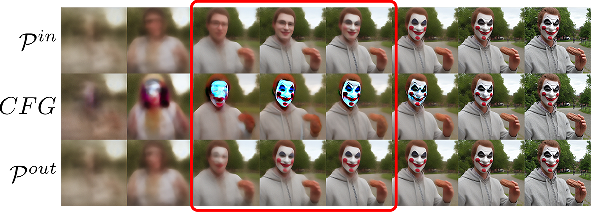
\includegraphics[width=0.8\linewidth]{fig/CFG.pdf}

   \caption{
      Positive and Negative prompt $\hat \vz_0$ estimation across timesteps. We visualize the estimated $\hat \vz_0$ for positive $\pout$, negative prompt $\pin$, and CFG  (both $\pout$ and $\pin$) during DDIM sampling with CFG.
   }
   \label{fig:posneg_direction}
\end{figure}

\subsection{Self-Attention Guidance}
\label{sec:self_attention_guidance}

{\modified{}This paper proposes} two complementary guidance mechanisms to simultaneously achieve effective editing—altering the image to match the target prompt $\pout$—and faithful reconstruction—preserving key regions of the input image.

For editing, {\modified{}a variant of classifier-free guidance (CFG) is adopted} \cite{miyake2023negative}

\begin{align}
  \label{eq:cfg}
    \begin{split}
      \tilde{\varepsilon}_{\theta}^{t}(\vz_{t},&\pin,\pout)= \varepsilon_{\theta}^{t}(\vz_{t},\pin)\\
      &+ w \cdot \left( \varepsilon_{\theta}^{t}(\vz_{t},\pout) - \varepsilon_{\theta}^{t}(\vz_{t},\pin) \right) 
    \end{split}
\end{align}
with $w>0$ modulating the balance between the two objectives. As illustrated in Fig.~\ref{fig:posneg_direction}, early in the diffusion process, the noise estimates for $\pin$ and $\pout$ both steer $\hat{\vz}_t$ toward the original image; then diverge: $\varepsilon_{\theta}^{t}(\vz_{t},\pin)$ favors reconstruction while $\varepsilon_{\theta}^{t}(\vz_{t},\pout)$ drives the editing transformation. 
As $t$ approaches 1, these estimates converge, resulting in a final image that balances input fidelity with the desired prompt edits.
In practice, an excessively low $w$ results in over-reconstruction, whereas a very high $w$ may neglect crucial details of the input image.

To promote reconstruction without resorting to explicit optimization or direct latent-space comparisons (which can cause diffusion instability), {\modified{}the proposed method leverages} the self-attention maps within the U-Net architecture. Unlike cross-attention—which only associates textual tokens with specific image regions \cite{hertz2023prompt,han2023proximal}—self-attention encodes global interactions among all image tokens, capturing richer spatial relationships that are essential for preserving image details not explicitly mentioned in the prompt. Concretely, during DDIM inversion, {\modified{}self-attention maps} $S_{i,t}^{in}$ {\modified{}are recorded} for each transformer block, and during synthesis, {\modified{}corresponding maps} $S_{i,t}^{out}$ {\modified{}are collected} from $\varepsilon_{\theta}^{t}(\vz_{t},\pout)$. {\modified{}Reconstruction is then enforced} by minimizing the loss
\begin{equation}
    \label{eq:self_attention_guidance}
    \mathcal{L}^\text{self}_t =  \sum^N_i \|S_{t,i}^{in} - S_{t,i}^{out}\|_1.
\end{equation}
This loss gradient, scaled by a factor $\lambda$, is incorporated into the noise update
\begin{equation}
    \hat{\vz}_{t-1} = \vz_{t-1} - \lambda \nabla_{\vz_t}\mathcal{L}^\text{self}_t.
\end{equation}
Following \cite{couairon2023monotonical}, {\modified{}factor} $\lambda$ progressively decreases with $t$, so that early diffusion steps emphasize the editing transformation while later steps focus on denoising and fine reconstruction.

In contrast to existing methods that require explicit reconstruction optimization \cite{mokady2023null,miyake2023negative} or depend solely on cross-attention for guidance, {\modified{}the presented approach integrates} self-attention guidance to capture all necessary information from the DDIM inversion. This strategy not only stabilizes the reverse diffusion process but also achieves a more robust and balanced trade-off between editing and reconstruction, thereby differentiating {\modified{}this contribution} from prior work.

% \setlength{\tabcolsep}{1pt}
\begin{figure}[h]
    \small
    \centering
    \begin{tabular}{ccc}
      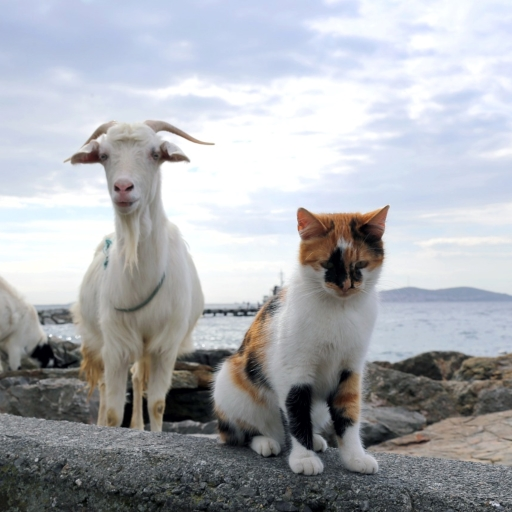
\includegraphics[width=1.8cm, height=1.8cm]{fig/cross_map_images/cross_image} & 
\includegraphics[width=1.8cm, height=1.8cm]{fig/cross_map_images/cat_map} & 
\includegraphics[width=1.8cm, height=1.8cm]{fig/cross_map_images/goat_map} \\
      Input & \textit{``cat"} & \textit{``goat"} \\
    %   \multicolumn{3}{c}{``\textit{a \textcolor{BrickRed}{\st{man}} \textcolor{RoyalBlue}{\textbf{woman}} smiling}"} \\
    %   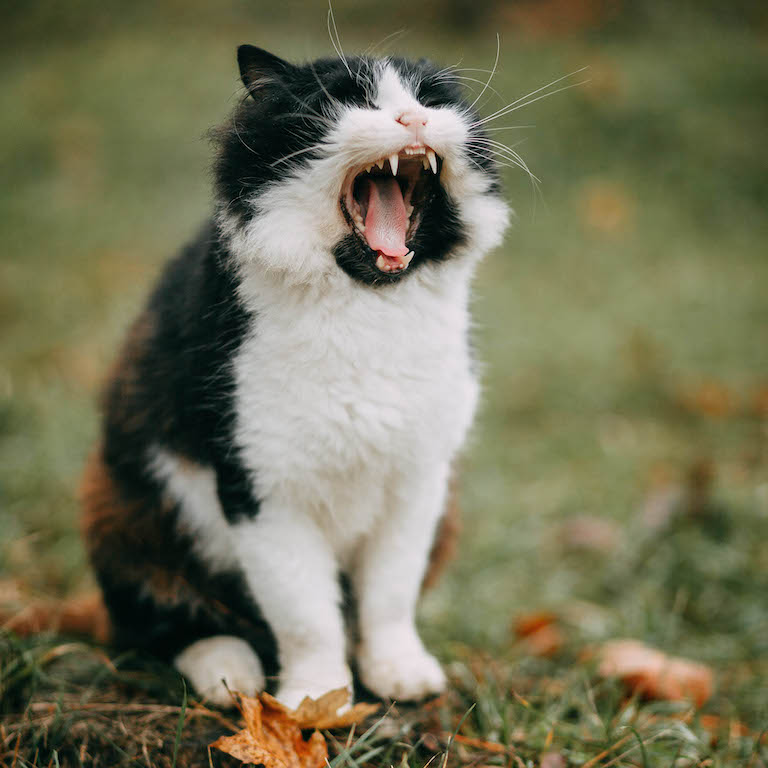
\includegraphics[width=2.2cm, height=2.2cm]{fig/teaser/teaser_2_in.jpg} & $\rightarrow$ & 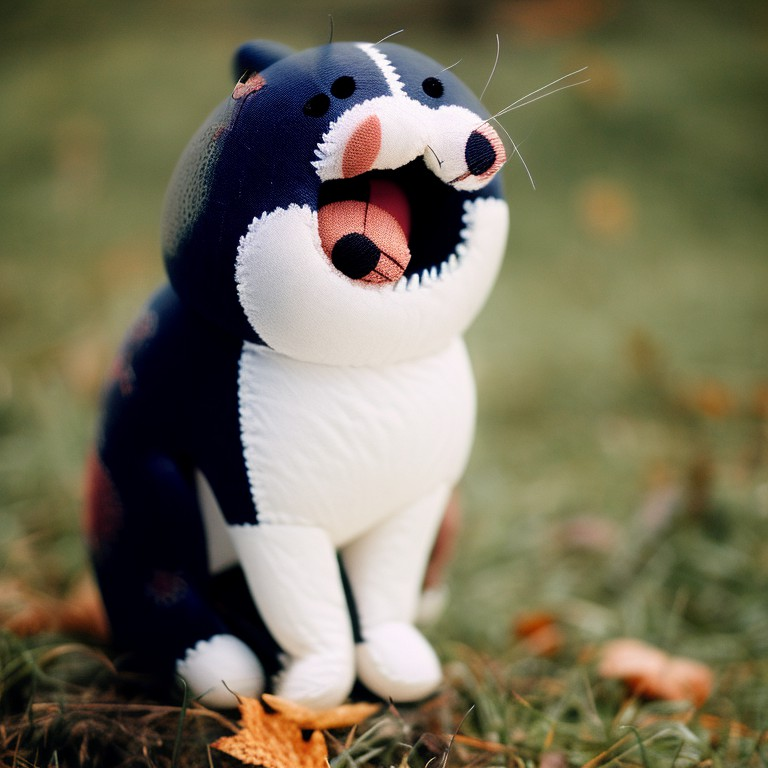
\includegraphics[width=2.2cm, height=2.2cm]{fig/teaser/teaser_2_out} \\
    %   \multicolumn{3}{c}{``\textit{a \textcolor{RoyalBlue}{\textbf{plush toy}} cat yawning }"} \\
      
    \end{tabular}
    \caption{Averaged $16 \times 16$ cross-attention maps corresponding to ``\textit{cat}" and ``\textit{goat}" for the input ``\textit{A cat and a goat}."}
    \label{fig:crossatt_map}
  \end{figure}

%   \begin{figure}
%     \includegraphics[width=0.99\linewidth]{fig/03_bird_and_bear.pdf}
%     \caption{Averaged cross-attention maps for the sentence "a furry bear watching a bird". The cross-attention maps corresponding to \textit{bird} and \textit{bear} are also shown across different timesteps. Figure taken from \cite{hertz2023prompt}. \guille{This is 100\% stolen from prompt-to-prompt but I believe it's really important for understanding what cross-attention maps are and what do they encode. How critital is that we make our own?}}
%     \label{fig:crossattn_viz}
%   \end{figure}
  


\subsection{Cross-Attention Manipulation}
\label{sec:cross_attention_manipulation}
Following \cite{hertz2023prompt} (see also \cite{mokady2023null,parmar2023zero,han2023proximal,ju2023direct,miyake2023negative}), {\modified{}this method uses} the U-Net’s cross-attention maps—which link latent space coordinates to prompt tokens—to guide the structural editing process. {\modified{}Proposed} adaptations include three mechanisms:


\textbf{Local Blending.} To recover fine details (e.g., colors and textures) that may be lost with self-attention alone, {\modified{}a high-resolution blending mask is derived} from the cross-attention maps. {\modified{}The maps from both the original prompt} $\pin$ and the editing prompt $\pout$ {\modified{}are aggregated} across diffusion steps and U-Net layers, then normalized, thresholded, and upscaled to obtain a binary mask $M$. This mask is used to fuse the edited latent $\vz_{t-1}$ with the original latent $\zddim_{t-1}$

\begin{equation}
    \label{eq:local_blend}
    \hat{\vz}_{t-1} = M \odot \vz_{t-1} + (1-M) \odot \zddim_{t-1}.
\end{equation}
This approach enhances detail preservation and improves computational efficiency by leveraging a single CFG estimation.

\textbf{Cross-Attention Replacement.} When $\pout$ involves a word swap in $\pin$, {\modified{}the shape of the modified object is preserved} by replacing the cross-attention maps for the altered token. Specifically, for token $k$, {\modified{}the method substitutes} $C_{t,i}^{out}[k]$ with $C_{t,i}^{in}[k]$ during the early diffusion stages (roughly the first 20\%), balancing shape retention with overall image quality.

\textbf{Cross-Attention Reweighting.} Finally, users can adjust the influence of specific words by reweighting the corresponding cross-attention maps $C_{t,i}^{out}[k]$, offering fine-grained control over the editing outcome.

These mechanisms, derived with minor adaptations from \cite{hertz2023prompt}, complement {\modified{}the presented framework} by refining structural guidance and detail preservation during image synthesis.
